% --------------------------------------------------------------------------------

\begin{exercise}

In Example 4.1, suppose a new state $15$ is added to the gridworld just below state $13$, and its actions, $\mathit{left}, \mathit{up}$ $\mathit{right}$, and $\mathit{down}$, take the agent to states $12$, $13$, $14$, and $15$, respectively.
Assume that the transistions from the original states are unchnged. 
What, the, ist $v_\pi(15)$ for the equiprobable random policy?
Now suppose the dynamics of state $13$ are also changed, such that action down from state $13$ takes the agent to the new state $15$.
What is $v_\pi(15)$ for the equiprobable random policy in this case?

\end{exercise}

% --------------------------------------------------------------------------------

\begin{solution}

\phantom{}

\begin{enumerate}[label = \arabic*.]

    \item Part:
    
    We formally define

    \begin{align*}
        \mathcal A(15)
        :=
        \Bbraces
        {
            \mathit{left},
            \mathit{up},
            \mathit{right},
            \mathit{down}
        }.
    \end{align*}

    Now, we know that the Bellman equations (3.14), from \cite*[page 59]{SuttonRichardS2018Rl:a}, have to apply.

    \begin{align*}
        v_\pi(15)
        & =
        \sum_{a \in \mathcal A(s)}
            \pi(a \mid 15)
            \sum_{\substack{s^\prime \in \mathcal S \cup \Bbraces{15} \\ r \in \mathcal R}}
                p(s^\prime, r \mid 15, a)
                \bbraces{r + \gamma v_\pi(s^\prime)} \\
        & =
        \frac{1}{4}
        (
            -1 + \gamma v_\pi(12)
        )
        +
        \frac{1}{4}
        (
            -1 + \gamma v_\pi(13)
        )
        +
        \frac{1}{4}
        (
            -1 + \gamma v_\pi(14)
        )
        +
        \frac{1}{4}
        (
            -1 + \gamma v_\pi(15)
        ) \\
        & =
        \frac{\gamma}{4}
        (
            v_\pi(12) + v_\pi(13) + v_\pi(14)
        )
        +
        \frac{\gamma}{4}
        v_\pi(15)
        -
        4
        \frac{1}{4}
    \end{align*}

    \begin{align*}
        \iff
        \frac{\gamma}{4}
        (
            v_\pi(12) + v_\pi(13) + v_\pi(14)
        )
        -
        1
        & =
        v_\pi(15) - \frac{\gamma}{4} v_\pi(15) \\
        & =
        \pbraces
        {
            1 - \frac{\gamma}{4}
        }
        v_\pi(15)
    \end{align*}

    \begin{align*}
        v_\pi(15)
        & =
        \frac
        {
            \frac{\gamma}{4}
            (
                v_\pi(12) + v_\pi(13) + v_\pi(14)
            )
            -
            1
        }{
            1 - \frac{\gamma}{4}
        } \\
        & =
        \frac
        {
            \gamma (-22 - 20 - 14) - 4
        }{
            4 - \gamma
        } \\
        & =
        \frac{56 \gamma + 4}{\gamma - 4} \\
        & =
        \begin{cases}
            -1,  & \gamma = 0, \\
            -20, & \gamma = 1
        \end{cases}
    \end{align*}

    \begin{figure}[H]
        \centering
        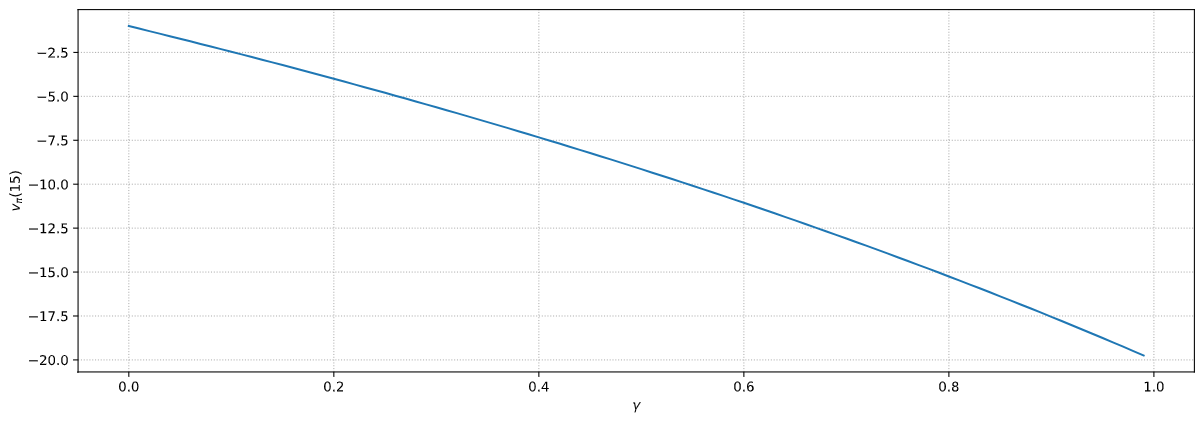
\includegraphics[width = 0.75 \textwidth]{3.23.png}
        \caption{}
        \label{fig:2.23}
    \end{figure}

    \item Part:
    
    \begin{align*}
        v_{\pi, \text{old}}(s)
        & =
        \sum_{a \in \mathcal A(s)}
            \pi(a \mid s)
            \sum_{\substack{s^\prime \in \mathcal S \cup \Bbraces{15} \\ r \in \mathcal R}}
                p_\text{old}(s^\prime, r \mid s, a)
                \bbraces{r + \gamma v_{\pi, \text{old}}(s^\prime)} \\
        & =
        \sum_{a \in \mathcal A(s) \setminus \Bbraces{\mathit{down}}}
            \pi(a \mid s)
            \sum_{\substack{s^\prime \in \mathcal S \cup \Bbraces{15} \\ r \in \mathcal R}}
                p_\text{old}(s^\prime, r \mid s, a)
                \bbraces{r + \gamma v_{\pi, \text{old}}(s^\prime)} \\
        & +
        \pi(\mathit{down} \mid s)
        \sum_{r \in \mathcal R}
            \Bigg (
                \sum_{s^\prime \in \mathcal S \setminus \Bbraces{13}}
                    p_\text{old}(s^\prime, r \mid s, \mathit{down})
                    \bbraces{r + \gamma v_{\pi, \text{old}}(s^\prime)} \\
                & +
                p_\text{old}(13, r \mid s, \mathit{down})
                \bbraces{r + \gamma v_{\pi, \text{old}}(13)}
                +
                p_\text{old}(15, r \mid s, \mathit{down})
                \bbraces{r + \gamma v_{\pi, \text{old}}(15)}
            \Bigg ) \\
        & =
        \sum_{a \in \mathcal A(s) \setminus \Bbraces{\mathit{down}}}
            \pi(a \mid s)
            \sum_{\substack{s^\prime \in \mathcal S \cup \Bbraces{15} \\ r \in \mathcal R}}
                p_\text{old}(s^\prime, r \mid s, a)
                \bbraces{r + \gamma v_{\pi, \text{old}}(s^\prime)} \\
        & +
        \pi(\mathit{down} \mid s)
        \sum_{r \in \mathcal R}
            \Bigg (
                \sum_{s^\prime \in \mathcal S \setminus \Bbraces{13}}
                    p_\text{old}(s^\prime, r \mid s, \mathit{down})
                    \bbraces{r + \gamma v_{\pi, \text{old}}(s^\prime)} \\
                & +
                (
                    p_\text{old}(13, r \mid s, \mathit{down})
                    +
                    p_\text{old}(15, r \mid s, \mathit{down})
                )
                \bbraces{r + \gamma (-20)}
            \Bigg ) \\
        & \stackrel{!}{=}
        \sum_{a \in \mathcal A(s) \setminus \Bbraces{\mathit{down}}}
            \pi(a \mid s)
            \sum_{\substack{s^\prime \in \mathcal S \cup \Bbraces{15} \\ r \in \mathcal R}}
                p_\text{new}(s^\prime, r \mid s, a)
                \bbraces{r + \gamma v_{\pi, \text{new}}(s^\prime)} \\
        & +
        \pi(\mathit{down} \mid s)
        \sum_{r \in \mathcal R}
            \Bigg (
                \sum_{s^\prime \in \mathcal S \setminus \Bbraces{13}}
                    p_\text{new}(s^\prime, r \mid s, \mathit{down})
                    \bbraces{r + \gamma v_{\pi, \text{new}}(s^\prime)} \\
                & +
                (
                    p_\text{new}(13, r \mid s, \mathit{down})
                    +
                    p_\text{new}(15, r \mid s, \mathit{down})
                )
                \bbraces{r + \gamma (-20)}
            \Bigg ) \\
        & \stackrel{!!}{=}
        \sum_{a \in \mathcal A(s) \setminus \Bbraces{\mathit{down}}}
            \pi(a \mid s)
            \sum_{\substack{s^\prime \in \mathcal S \cup \Bbraces{15} \\ r \in \mathcal R}}
                p_\text{new}(s^\prime, r \mid s, a)
                \bbraces{r + \gamma v_{\pi, \text{new}}(s^\prime)} \\
        & +
        \pi(\mathit{down} \mid s)
        \sum_{r \in \mathcal R}
            \Bigg (
                \sum_{s^\prime \in \mathcal S \setminus \Bbraces{13}}
                    p_\text{new}(s^\prime, r \mid s, \mathit{down})
                    \bbraces{r + \gamma v_{\pi, \text{new}}(s^\prime)} \\
                & +
                p_\text{new}(13, r \mid s, \mathit{down})
                \bbraces{r + \gamma v_{\pi, \text{new}}(13)}
                +
                p_\text{new}(15, r \mid s, \mathit{down})
                \bbraces{r + \gamma v_{\pi, \text{new}}(15)}
            \Bigg ) \\
        & =
        \sum_{a \in \mathcal A(s)}
            \pi(a \mid s)
            \sum_{\substack{s^\prime \in \mathcal S \cup \Bbraces{15} \\ r \in \mathcal R}}
                p_\text{new}(s^\prime, r \mid s, a)
                \bbraces{r + \gamma v_{\pi, \text{new}}(s^\prime)} \\
        & =
        v_{\pi, \text{new}}(s)
    \end{align*}

    \Quote{!} follows from

    \begin{align*}
        p_\text{old}(13, r \mid s, \mathit{down})
        +
        p_\text{old}(15, r \mid s, \mathit{down})
        =
        p_\text{new}(13, r \mid s, \mathit{down})
        +
        p_\text{new}(15, r \mid s, \mathit{down}).
    \end{align*}

    For \Quote{!} we used the Ansatz $v_{\pi, \text{new}} \doteq v_{\pi, \text{old}}$, which checks out in the end, by virtue of the Bellman equation's unique solvability.

\end{enumerate}

\end{solution}

% --------------------------------------------------------------------------------
